\chapter{Generalised Linear Models}
\label{chap:GLM}

Aims of this chapter\footnote{Here you work with the script file {\tt glm.R}}:
\begin{compactitem}
	\item Use generalised linear models (GLMs) to handle count data.
	\item Analyse some genetics practical data.
	\item This chapter will step through the analysis carefully. These 
	are not simple analyses so you should concentrate on understanding 
	the process and the biology and think about how to present your 
	results.
	
\end{compactitem}

\section{What is a GLM?}

the generalized linear model (GLM) is a generalization of ordinary 
linear regression analyses to accommodate response variables to have 
non-normal error distributions (e.g., count data, as in the genetics 
practical data --- see below).

\section{The data}

We will use mutation data collected by a previous year's batch in the 
Genetics Practical. So let's actually use some of the skills you've 
learned to do some statistical modelling on data you might collect. 
That is, you  can aim to repeat these analyses with similar data you 
collect.

The students were basically counting colonies looking for mutations. 
There were a number of bacterial strains which were different mutants 
of {\it Salmonella}. Each group applied a mutagen Nitroguanisine (NG) 
as well as histidine and streptomycine. A control plate was also 
tested. 

The data file in CSV format is available from the bitbucket site, as 
usual in the {\tt Data} directory. It is called {\tt PracData.csv}.

\begin{compactitem}[$\quad\star$]
	\item Save the {\tt PracData.csv} dataset into your {\tt Data} 
	directory. 
	\item Create a new script called MyGLM in your {\tt Code} directory.  
	Use the code below to load and check your data.
	\item Start R and change the working directory to {\tt Code}.
\end{compactitem}

\begin{lstlisting}
> colonies <- read.csv("../Data/PracData.csv")
> str(colonies)

 'data.frame':	680 obs. of  5 variables:
 $Student.ID : Factor w/ 34 levels "A1","A10","A11",..: 1 1 1 2 2 2 4 4 4 4 ...
 $Strain     : Factor w/ 5 levels "421","712","881",..: 4 3 5 1 2 3 4 2 3 5 ...
 $Treatment  : Factor w/ 4 levels "Control","His",..: 1 1 1 3 3 1 1 3 3 1 ...
 $ColonyCount: int  0 0 0 0 0 0 0 0 0 0 ...
 $HaloLawn   : Factor w/ 2 levels "N","Y": NA NA NA NA NA NA NA NA NA NA ...
\end{lstlisting}

Now that we've got the data loaded, we need to look at it and try and 
see what is going on.

\section{Plotting the data}

We have a continuous response variable ({\tt ColonyCount}) and two 
categorical explanatory variables ({\tt Strain} and {\tt Treatment}). 
We also have observations of halos and bacterial lawns around the 
treated areas ({\tt HaloLawn}), which we will come back to at the end 
of this chapter.

So, with two factors as the explanatory variables, we will use box and 
whisker plots and boxplots to explore the data. First, we'll look at 
the effects of the four treatments.

\begin{lstlisting}
> boxplot(ColonyCount ~ Treatment, data=colonies)
\end{lstlisting}
	
\begin{center}
	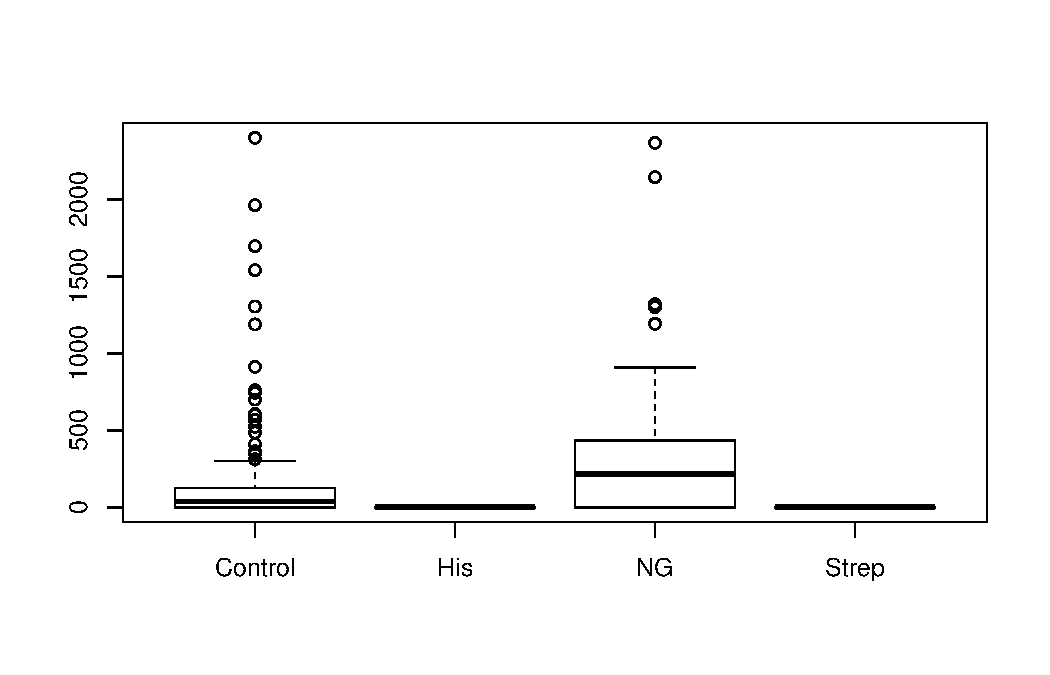
\includegraphics[width=0.6\textwidth]{Bxp.pdf}
\end{center}  

There are two immediate things to note. 
\begin{enumerate}

	\item The distributions of colony counts are very {\it skewed} --- 
	many small counts and a few large counts. We've already seen that 
	taking a log of data sometimes works in these cases. However, as the 
	tables above show, we have zero counts for all treatments and 
	$\log(0)$ is undefined. A common trick is therefore to use 
	$\log(n+1)$ (add 1 and take a log) when dealing with count data like 
	this:

\begin{lstlisting}
> colonies$logCC <- log(colonies$ColonyCount + 1)
> boxplot(logCC ~ Treatment, data=colonies)
\end{lstlisting}

\begin{center}
	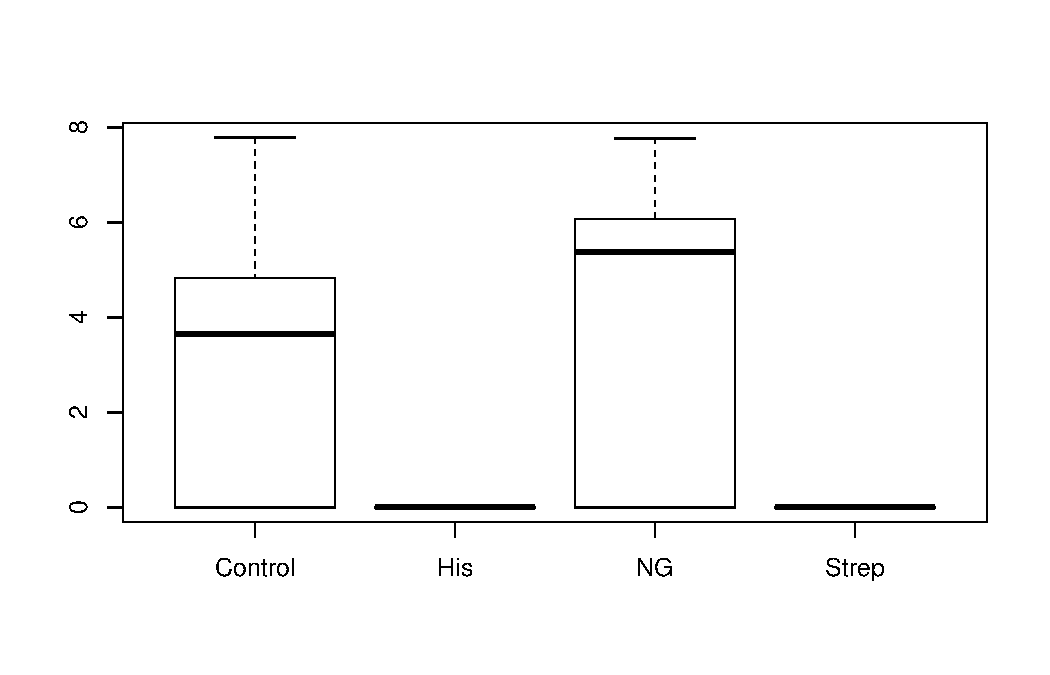
\includegraphics[width=0.6\textwidth]{logBxp.pdf} 
\end{center}

I hope you'll agree that this still doesn't look very convincingly like 
normal data, but we'll come back to this point. 

	\item The colony counts are vastly different between the different 
	treatments. It is hard to say for sure from the two plots, but it looks 
	like colonies never grow under the histidine and streptomycine 
	treatments. We can check that:

\begin{lstlisting}
> tapply(colonies$ColonyCount, colonies$Treatment, min, na.rm = TRUE)

 Control     His      NG   Strep 
       0       0       0       0 

> tapply(colonies$ColonyCount, colonies$Treatment, max, na.rm = TRUE)

 Control     His      NG   Strep 
    2400       0    2367       0 
\end{lstlisting}

There is indeed no variation at all in colony count for histidine and 
streptomycine --- colonies never grow in these treatments. We don't 
really need statistics for this observation and, in fact, variation is 
needed for statistics to work. So, for the rest of this analysis, we 
will reduce the dataset to the control and nitroguanisine treatments. 

\end{enumerate}

\begin{compactitem}[$\quad\star$]
	\item Update your script to contain the code for these plots.
\end{compactitem}

We'll use a new piece of code here to get the right subset. {\tt var 
\%in\% c('a','b','c')} finds all entries in {\tt var} whose values are 
equal to {\tt 'a'},  {\tt 'b'} or  {\tt 'c'}.

\begin{lstlisting}
> coloniesCN <- subset(colonies, Treatment %in% c("Control", "NG"), 
drop = TRUE) 
> str(coloniesCN)

 'data.frame':	340 obs. of  6 variables:
 $Student.ID : Factor w/ 34 levels "A1","A10","A11",..: 1 1 1 2 2 2 4 4 4 4 ...
 $Strain     : Factor w/ 5 levels "421","712","881",..: 4 3 5 1 2 3 4 2 3 5 ...
 $Treatment  : Factor w/ 4 levels "Control","His",..: 1 1 1 3 3 1 1 3 3 1 ...
 $ColonyCount: int  0 0 0 0 0 0 0 0 0 0 ...
 $HaloLawn   : Factor w/ 2 levels "N","Y": NA NA NA NA NA NA NA NA NA NA ...
 $logCC      : num  0 0 0 0 0 0 0 0 0 0 ...
\end{lstlisting}

You'll see that, although we have removed two treatments, their names 
still appear in the list of levels in the {\tt str} output. R retains a 
list of all the levels that were originally in a factor, even when 
those levels aren't used any more. This will be annoying later, so 
we'll use the {\tt droplevels} function to strip them out.

\begin{lstlisting}
> coloniesCN <- droplevels(coloniesCN)
> str(coloniesCN)

 'data.frame':	340 obs. of  6 variables:
 $Student.ID : Factor w/ 34 levels "A1","A10","A11",..: 1 1 1 2 2 2 4 4 4 4 ...
 $Strain     : Factor w/ 5 levels "421","712","881",..: 4 3 5 1 2 3 4 2 3 5 ...
 $Treatment  : Factor w/ 2 levels "Control","NG": 1 1 1 2 2 1 1 2 2 1 ...
 $ColonyCount: int  0 0 0 0 0 0 0 0 0 0 ...
 $HaloLawn   : Factor w/ 0 levels: NA NA NA NA NA NA NA NA NA NA ...
 $logCC      : num  0 0 0 0 0 0 0 0 0 0 ...
\end{lstlisting}

\begin{compactitem}[$\quad\star$]
	\item Add these commands to subset your data to your code file.
\end{compactitem}

\section{Looking at strains too}

Now we'll look to see how counts differ between the strains.  A simple 
way to visualise this is to use the {\tt lattice} package again to get 
plots grouped by treatment.

\begin{lstlisting}
> library(lattice) 
> bwplot(logCC ~ Strain | Treatment, data=coloniesCN)
\end{lstlisting}

\begin{center}
	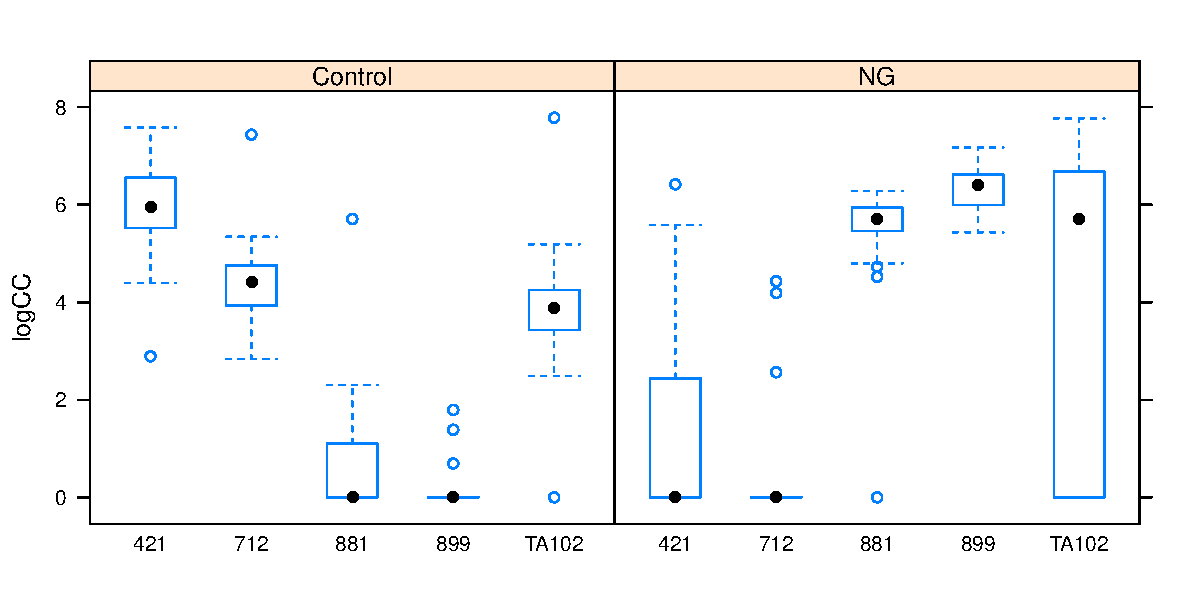
\includegraphics[width=\textwidth]{GLM_lattice.pdf}	
\end{center}

First impressions from this figure:
\begin{enumerate}
	\item The strains are doing {\it very} different things under the two 
	treatments. Hopefully this now leaps out at you as suggesting that 
	the two variables (Strain and Treatment) are {\it interacting}. \item 
	The distributions are still pretty ugly --- the variances differ 
	hugely between combinations and four combinations have a median of 
	zero.
\end{enumerate}

We could also use a barplot of means here. We'll use the original data 
to get the means, but can use a log scale on the $y$ axis ({\tt 
log='y'}).

\begin{lstlisting}
> tab <- tapply(coloniesCN$ColonyCount, list(coloniesCN$Treatment,
coloniesCN$Strain), mean, na.rm=TRUE)
> print(tab)

            421     712    881     899 TA102
 Control 538.20 138.867  12.73   0.375 126.7
 NG       61.29   5.517 292.71 593.000 523.9
\end{lstlisting}

An then, 

\begin{lstlisting}
> barplot(tab, beside=TRUE, log= ' y ' )	
\end{lstlisting}

Which should give,
\begin{center}
	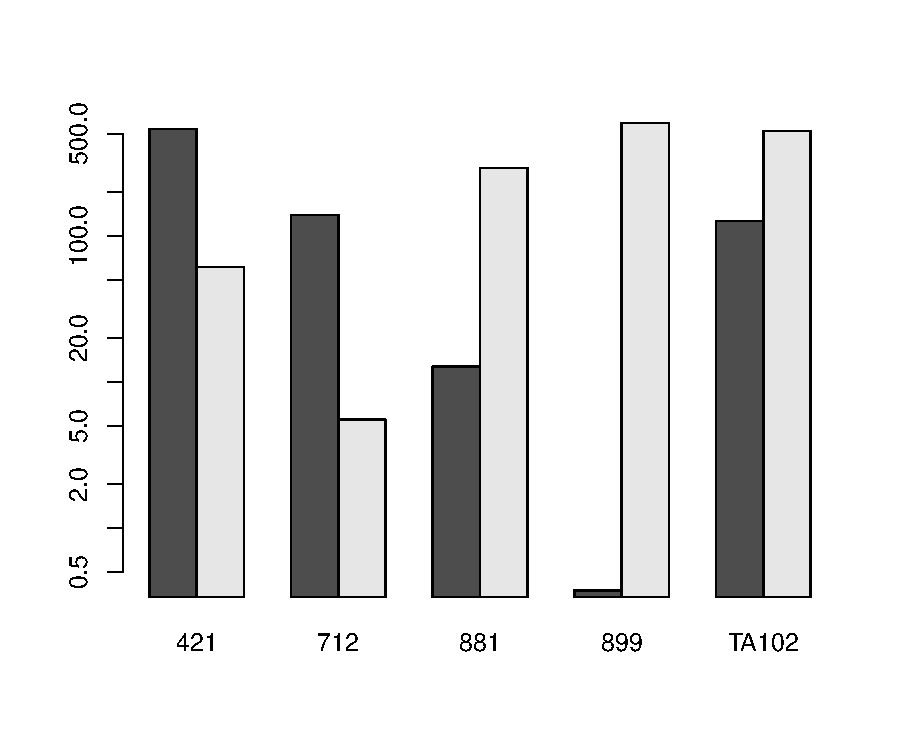
\includegraphics[width=0.6\textwidth]{GLM_barplot.pdf} 
\end{center}

Lets have a look at a first model.

\section{A linear model}

We'll fit a model of colony count as the interaction between strain and 
treatment and then look at the diagnostic plots. We'd do this anyway, 
but we're already suspicious about the variance.

\begin{lstlisting}
> modLM <- lm(logCC ~ Strain * Treatment, data=coloniesCN)
> par(mfrow=c(2,2), mar=c(3,3,3,1), mgp=c(2,0.8,0))
> plot(modLM)
\end{lstlisting}

\begin{center}
	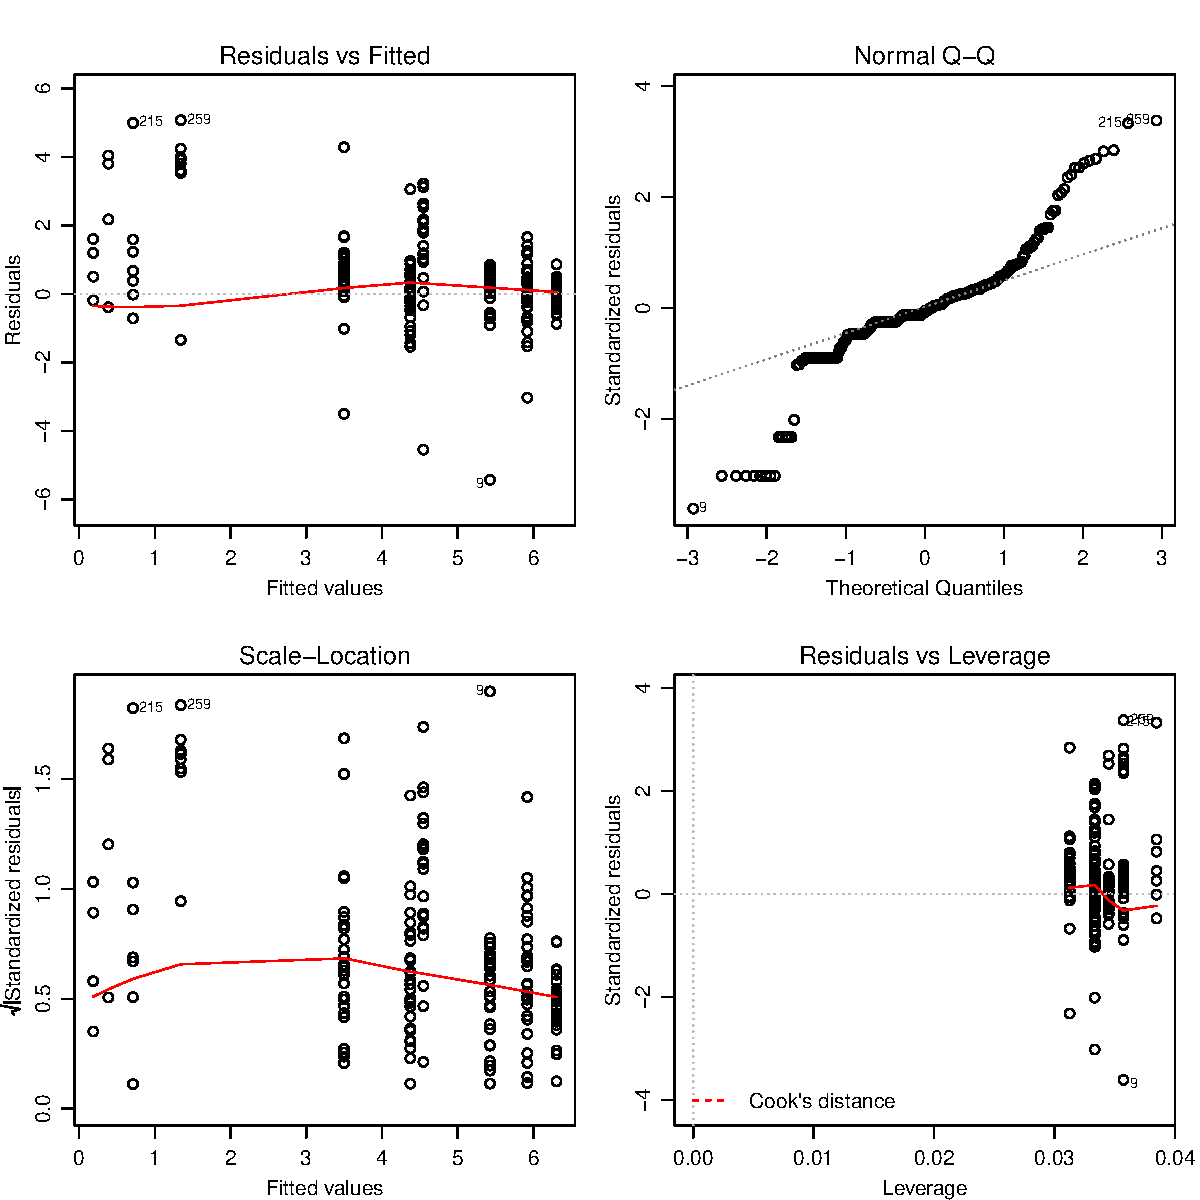
\includegraphics[width=\textwidth]{lmDisaster.pdf} 	
\end{center}

\begin{compactitem}[$\quad\star$]
	\item Run this code and have a close look at the plots. 
\end{compactitem}

That normal QQ plot is not good. Our suspicions were justified and it 
doesn't look like we can use a simple log transformation. We're not 
even going to look at the {\tt anova} and {\tt summary} tables --- if 
the diagnostic plots are bad enough, then the model outputs are not to 
be trusted.

\section{Generalised linear models}

In the linear models lecture, we looked at the expectation of {\it 
constant normal variance} in linear models. Whatever the combination of 
explanatory variables for a particular prediction, the residuals around 
that prediction have similar variance and are roughly normally 
distributed. The panel on the left shows this basic idea.

\begin{center}
	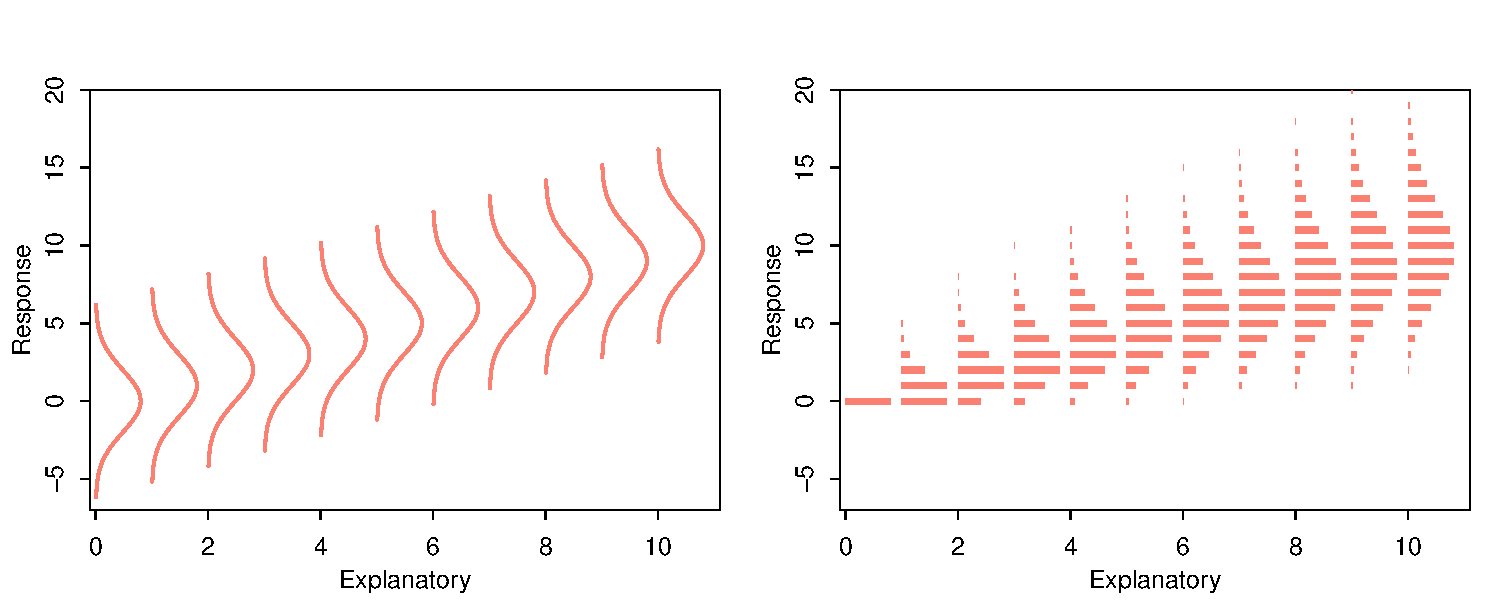
\includegraphics[width=\textwidth]{GLMexample.pdf} 
\end{center}

As we have seem, count data does not have this distribution, even when 
logged. The panel on the right shows the expected distribution of count 
data as the mean count increases with an explanatory  variable.  There 
are three key differences between the two panels:

\begin{enumerate}
	\item Counts can {\it never} be negative but can be zero.
	\item Counts are always {\it integers} --- whole numbers --- rather 
	than being continuous.
	\item The variance of count data is {\it not constant}. As the 
	average predicted count gets larger, so does the variance. Unlike the 
	normal distribution, where variance can take any value, for count 
	data  the variance is expected to be equal to the mean.
\end{enumerate}

So, we have data that is unsuitable for a linear model because it 
doesn't show constant normal variance. This is where generalised linear 
models come in --- we can change the model for the expected residuals 
to use a different distribution. For count data, this is the {\it 
Poisson} distribution.

We need to change the function we use to fit models to {\tt glm}, but 
otherwise the process is very similar. The whole point of the GLM is to 
model the original count data more appropriately, so we will abandon 
the logged data too. GLMs can cope with a range of different 
distributions, so we have to specify the {\tt family} of the 
distribution we want to use.

\begin{lstlisting}
> modPois <- glm(ColonyCount ~ Strain * Treatment, data=coloniesCN, 
family= 'poisson')
\end{lstlisting}

First, we'll look at the summary table for this model. We have 5 levels 
of strain and 2 levels of factor in the subset so we get an intercept 
($i$), 4 differences for strains($s_{2-5}$), one difference for 
treatment ($t_2$) and then four differences for the interaction 
($s_{2-5}t_2$). These combine like this:
 
\[\begin{array}{|l|c|c|}
\hline
							& \textrm{Control} & \textrm{Nitroguanisine} \\
\hline
\textrm{421}   & i        & i+t_2              \\
\textrm{712}   & i + s_2  & i+s_2+t_2+ s_2t_2  \\
\textrm{881}   & i + s_3  & i+s_3+t_2 + s_3t_2  \\
\textrm{889}   & i + s_4  & i+s_4+t_2 + s_4t_2  \\
\textrm{TA102} & i + s_5  & i+s_5+t_2  + s_5t_2 \\
\hline
\end{array}\]

The summary table looks like this --- very similar to the {\tt summary} 
table for a linear model.

\begin{lstlisting}
> summary(modPois)
 
 Call:
 glm(formula = ColonyCount ~ Strain * Treatment, family = "poisson", 
     data = coloniesCN)
 
 Deviance Residuals: 
    Min      1Q  Median      3Q     Max  
 -32.37  -10.33   -3.32    0.84   97.84  
 
 Coefficients:
                         Estimate Std. Error z value Pr(>|z|)    
 (Intercept)              6.28823    0.00787   799.0   <2e-16 ***
 Strain712               -1.35472    0.01738   -78.0   <2e-16 ***
 Strain881               -3.74421    0.05549   -67.5   <2e-16 ***
 Strain899               -7.26906    0.28878   -25.2   <2e-16 ***
 StrainTA102             -1.44651    0.01757   -82.3   <2e-16 ***
 TreatmentNG             -2.17268    0.02539   -85.6   <2e-16 ***
 Strain712:TreatmentNG   -1.05295    0.08446   -12.5   <2e-16 ***
 Strain881:TreatmentNG    5.30786    0.06152    86.3   <2e-16 ***
 Strain899:TreatmentNG    9.53871    0.28989    32.9   <2e-16 ***
 StrainTA102:TreatmentNG  3.59226    0.03090   116.2   <2e-16 ***
 ---
 Signif. codes:  0 '***' 0.001 '**' 0.01 '*' 0.05 '.' 0.1 ' ' 1 
 
 (Dispersion parameter for poisson family taken to be 1)
 
     Null deviance: 134445  on 293  degrees of freedom
 Residual deviance:  61579  on 284  degrees of freedom
   (46 observations deleted due to missingness)
 AIC: 62910
 
 Number of Fisher Scoring iterations: 7
 
\end{lstlisting}

So, interpreting this table quickly. Under the control treatment, 
strain 421 (the intercept) has the highest number of colonies and all 
the other strains have lower numbers to some degree --- the differences 
are negative. The overall effect of nitrogaunasine is to decrease the 
number of colonies --- again a negative coefficient --- but then the 
positive interactions show big increases in colony counts for 
nitroguanisine for specific strains. Everything is hugely significant.

\begin{compactitem}[$\quad\star$]
	\item Copy the code in this section into your script and explore the 
	model.
\end{compactitem}

\section{Overdispersion}

There's a problem. You may have already spotted it:

\begin{lstlisting}
> par(mfrow = c(2, 2), mar = c(3, 3, 3, 1), mgp = c(2, 0.8, 0))
> plot(modPois)
\end{lstlisting}

\begin{center}
	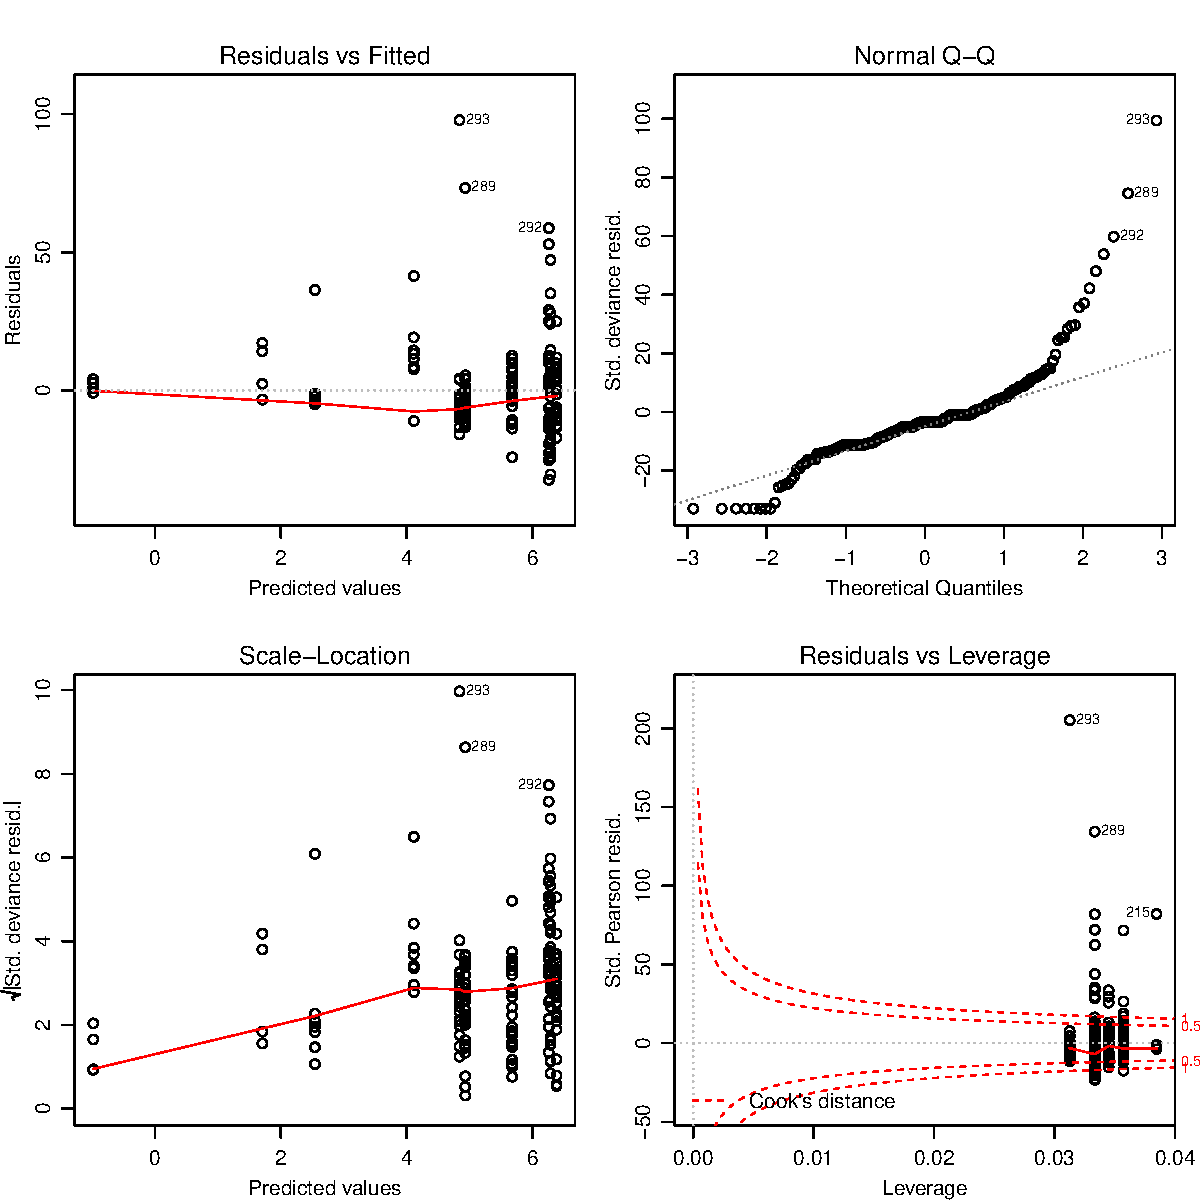
\includegraphics[width=0.8\textwidth]{poisDiag.pdf}
\end{center}

Actually, there are two problems. First, that QQ plot is still a bit 
dubious. More of the points are close to the line than in the linear 
model but there are some extreme positive residuals. Second, the 
magnitude of the residuals is enormous, and this is really clear in the 
plot in the bottom right hand corner. This plot identifies outliers and 
any points outside of the red dotted line are possible problems.

The problem here is {\it overdispersion}. The Poisson distribution 
predicts that the variance at a point in the model is equal to the 
prediction --- the mean count at that point. Our count data shows much 
more variance than this --- particularly that there are some huge 
counts given the means.

There is a simple way to check the dispersion of count data using the 
{\tt summary} table: the ratio of the residual deviance to the residual 
degrees of freedom should be approximately 1. This expectation is 
actually given in the table:

{\tt (Dispersion parameter for poisson family taken to be 1)}

In this case,  the ratio is $61579/284=216.8$. That's very strongly 
overdispersed. Fortunately, we can allow for this by using a different 
model.

\section{Generalised linear models using quasipoisson}

The quasipoisson family uses the data to estimate the dispersion of the 
model, but is otherwise very similar to using the Poisson family.

\begin{lstlisting}
> modQPois <- glm(ColonyCount ~ Strain * Treatment, data=coloniesCN,
family= 'quasipoisson')
\end{lstlisting}

The summary table now looks like this:

\begin{lstlisting}
> summary(modQPois) 

 Call:
 glm(formula = ColonyCount ~ Strain * Treatment, family = "quasipoisson", 
     data = coloniesCN)
 
 Deviance Residuals: 
    Min      1Q  Median      3Q     Max  
 -32.37  -10.33   -3.32    0.84   97.84  
 
 Coefficients:
                         Estimate Std. Error t value Pr(>|t|)    
 (Intercept)                6.288      0.158   39.78  < 2e-16 ***
 Strain712                 -1.355      0.349   -3.88  0.00013 ***
 Strain881                 -3.744      1.115   -3.36  0.00089 ***
 Strain899                 -7.269      5.800   -1.25  0.21113    
 StrainTA102               -1.447      0.353   -4.10  5.4e-05 ***
 TreatmentNG               -2.173      0.510   -4.26  2.8e-05 ***
 Strain712:TreatmentNG     -1.053      1.696   -0.62  0.53529    
 Strain881:TreatmentNG      5.308      1.236    4.30  2.4e-05 ***
 Strain899:TreatmentNG      9.539      5.822    1.64  0.10246    
 StrainTA102:TreatmentNG    3.592      0.621    5.79  1.9e-08 ***
 ---
 Signif. codes:  0 '***' 0.001 '**' 0.01 '*' 0.05 '.' 0.1 ' ' 1 
 
 (Dispersion parameter for quasipoisson family taken to be 403.4)
 
     Null deviance: 134445  on 293  degrees of freedom
 Residual deviance:  61579  on 284  degrees of freedom
   (46 observations deleted due to missingness)
 AIC: NA
 
 Number of Fisher Scoring iterations: 7 
\end{lstlisting}

This is pretty similar to the previous table but there two differences. 
First, the dispersion parameter line has changed. Second, all the $p$ 
values have got less significant -- this is the effect of controlling 
for the overdispersion. 

We'll look at the model diagnostic plots next:

\begin{lstlisting}
> par(mfrow = c(2, 2), mar = c(3, 3, 3, 1), mgp = c(2, 0.8, 0))
> plot(modQPois)	
\end{lstlisting}

\begin{center}
	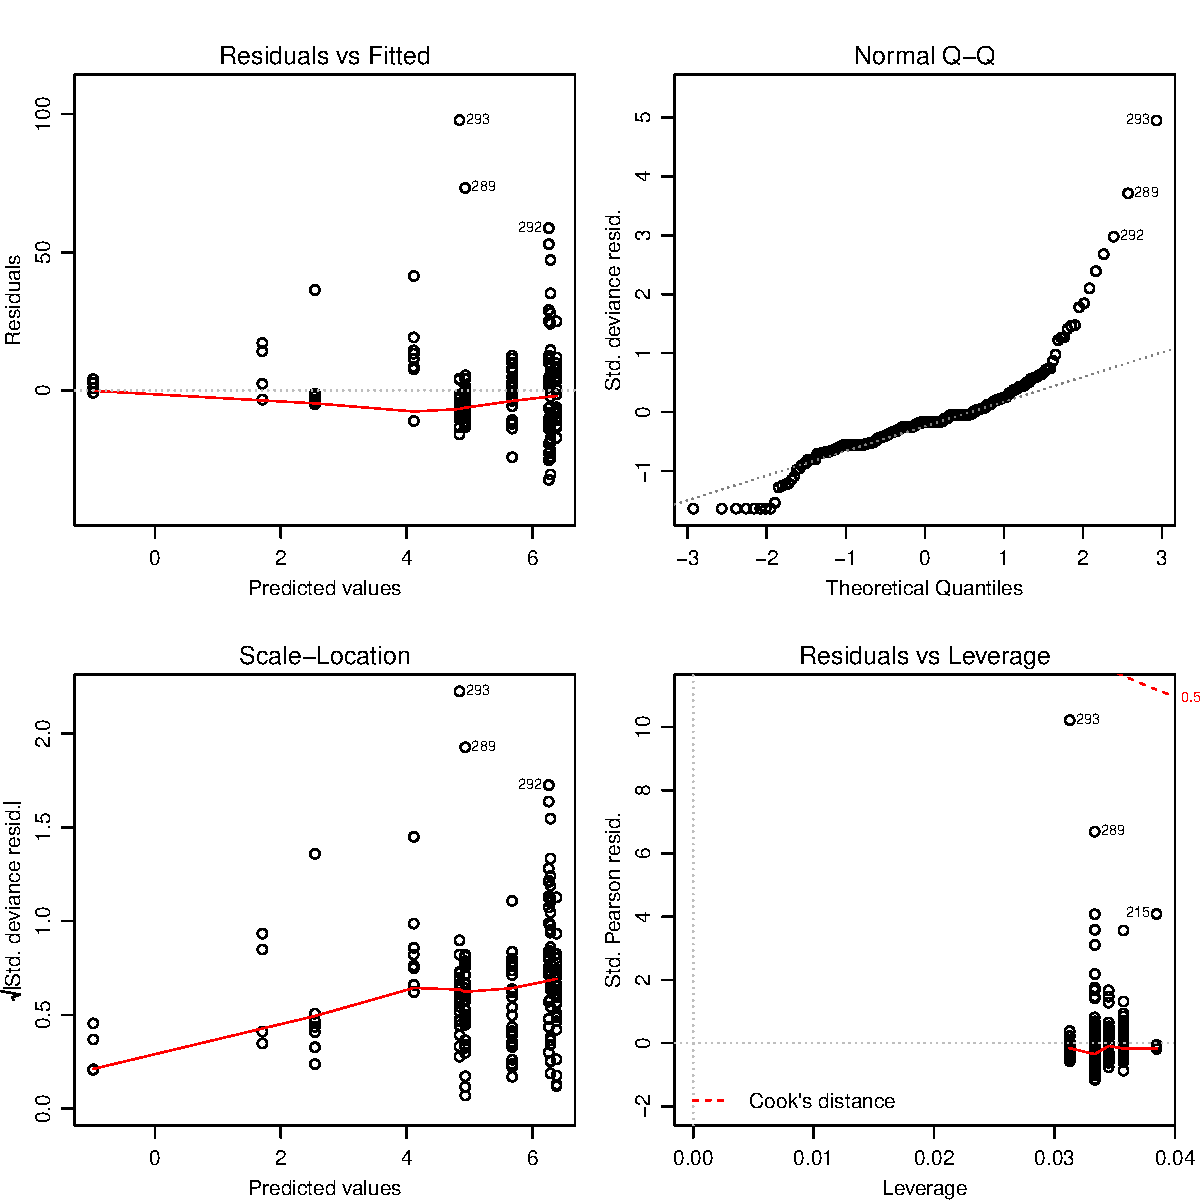
\includegraphics[width=0.8\textwidth]{qpoisDiag.pdf} 
\end{center}

The residuals and leverage plot is now ok. The QQ plot is not better, 
but is still an improvement over the original linear model. We can't 
improve the model fit any more ---  it isn't perfect but we'll accept 
those imperfections. It is worth thinking about the imperfections 
though --- what might give rise to occasional larger than expected 
counts of colonies?

We'll look at the {\tt anova} table next. Technically, this is now 
analysis of deviance not analysis of variance but the concept is the 
same. Different tests are appropriate for different families of 
distribution, but we can use $F$ here:

\begin{lstlisting}
> anova(modQPois, test = "F")

 Analysis of Deviance Table
 
 Model: quasipoisson, link: log
 
 Response: ColonyCount
 
 Terms added sequentially (first to last)
 
 
                  Df Deviance Resid. Df Resid. Dev     F  Pr(>F)    
 NULL                               293     134445                  
 Strain            4    13923       289     120521  8.63 1.4e-06 ***
 Treatment         1     6055       288     114467 15.01 0.00013 ***
 Strain:Treatment  4    52888       284      61579 32.78 < 2e-16 ***
 ---
 Signif. codes:  0 '***' 0.001 '**' 0.01 '*' 0.05 '.' 0.1 ' ' 1 
\end{lstlisting}

Can we simplify the model? The interaction is the only term we can drop 
and looks highly significant, but we can check by deleting it.

\begin{lstlisting}
> drop.scope(modQPois)

 [1] "Strain:Treatment"

> modQPois2 <- update(modQPois, . ~ . - Strain:Treatment)
> anova(modQPois, modQPois2, test = "F")

 Analysis of Deviance Table
 
 Model 1: ColonyCount ~ Strain * Treatment
 Model 2: ColonyCount ~ Strain + Treatment
   Resid. Df Resid. Dev Df Deviance    F Pr(>F)    
 1       284      61579                            
 2       288     114467 -4   -52888 32.8 <2e-16 ***
 ---
 Signif. codes:  0 '***' 0.001 '**' 0.01 '*' 0.05 '.' 0.1 ' ' 1 
\end{lstlisting}

No, that makes the model much worse, so we now have our final model. 

\begin{compactitem}[$\quad\star$]
	\item Fit this new model in your script and check you've got the same 
	results.
\end{compactitem}

\section{Model predictions}

We can get model predictions and standard errors using the {\tt 
predict} function. There is a difference though. GLMs use an internal 
transformation to model the data using a {\it link function} and the 
coefficients in the summary above are on the scale of the link 
transformation. For quasipoisson, this is a {\it log link}, which you 
can see in the output of {\tt anova}. You can use {\tt predict} to get 
predictions on the scale of the original {\it response}.

\begin{lstlisting}
# use expand.grid to get all combinations of factors
> df <- expand.grid(Strain = levels(coloniesCN$Strain), Treatment =
levels(coloniesCN$Treatment))
> predict(modQPois, newdata = df, type = "response")

       1       2       3       4       5       6       7       8       9      10 
 538.200 138.867  12.731   0.375 126.687  61.286   5.517 292.714 593.000 523.900 
\end{lstlisting}

Those are the same values as the means we calculated for the barplot. 
Adding standard errors to barplots is more difficult for GLMs and we 
won't go into it here.

\section{Reporting the model}

Reporting complicated statistics is a difficult business. There is a 
lot of detail involved and you want the reader to understand what you 
have done well enough to repeat the analysis if needed. You also have 
to summarise and explain the results without pages of R output. 

Here are some pointers:
\begin{itemize}
	\item What does the data show? Present a graph or a table to show the 
	data you are about to model. {\it Always} include a figure or table 
	legend and {\it always} refer to that figure or legend from the text.
	\item Have you transformed the data or used a subset? If so, why?
	\item What kind of model or statistical test have you used?
	\item With linear models, what is the response variable and what are 
	the explanatory variables.
	\item Have you simplified the model and, if so, what was the most 
	complex model you tried?
	\item How did you check the suitability of the model? Are there any 
	problems with the model and, if so, what might cause them?
	\item If you summarise stats in text, you must include all the 
	information about the test. 
	\begin{itemize}
		\item For $F$ tests, this is $F$, the two degrees of freedom and 
		the p value. For example: `There is a significant interaction 
		between treatment and strain ($F_{4,284}=32.7, p < 0.0001$)'. 
		\item For $t$ tests, this is the coefficient, the standard error, 
		$t$, the degrees of freedom and $p$. For example, `Across strains, 
		the main effect of nitroguanisine is to reduce colony counts 
		relative to the control (estimate=-2.17, s.e= 0.51, $t=-4.26$, 
		df=284,  $p < 0.0001$)'.
	\end{itemize}
	\item With more complex models, it is common to present either the 
	anova table or the coefficients table as a summary of the model 
	output. Just include the tables from R output, not the information 
	around it. See Table 1 for an example. 
	\item {\it Never} just include chunks of raw output from R.
	\item Most importantly, what is the interpretation of the model. What 
	is it telling you about the data?
\end{itemize}

{\it Table 1}: Coefficients from a GLM of treatment and strain as 
predictors of colony count.

% latex table generated in R 2.14.1 by xtable 1.7-0 package
% Wed Nov 28 08:56:01 2012
\begin{table}[ht]
	\begin{center}
		\begin{tabular}{rrrrl}
		  \hline
		 & Estimate & Std. Error & t value & p \\ 
		  \hline
		(Intercept) & 6.29 & 0.16 & 39.78 & <0.0001 \\ 
		  Strain712 & -1.35 & 0.35 & -3.88 & \phantom{<}0.0001 \\ 
		  Strain881 & -3.74 & 1.11 & -3.36 & \phantom{<}0.0009 \\ 
		  Strain899 & -7.27 & 5.80 & -1.25 & \phantom{<}0.2111 \\ 
		  StrainTA102 & -1.45 & 0.35 & -4.10 & <0.0001 \\ 
		  TreatmentNG & -2.17 & 0.51 & -4.26 & <0.0001 \\ 
		  Strain712:TreatmentNG & -1.05 & 1.70 & -0.62 & \phantom{<}0.5353 \\ 
		  Strain881:TreatmentNG & 5.31 & 1.24 & 4.30 & <0.0001 \\ 
		  Strain899:TreatmentNG & 9.54 & 5.82 & 1.64 & \phantom{<}0.1025 \\ 
		  StrainTA102:TreatmentNG & 3.59 & 0.62 & 5.79 & <0.0001 \\ 
		   \hline
		\end{tabular}
	\end{center}
\end{table}

\section{Halos and lawns}

We'll keep this one simple since it is harder to analyse. The response 
variable ({\tt HaloLawn}) is binary --- the plates either have a lawn 
or not. We'll just look at a contingency table of how many plates have 
halos or lawns under each combination of treatment and strain.

\begin{lstlisting}

> table(Halo = colonies$HaloLawn, Strain = colonies$Strain, Treatment = 
colonies$Treatment)

 , , Treatment = Control
 
     Strain
 Halo 421 712 881 899 TA102
    N   0   0   0   0     0
    Y   0   0   0   0     0
 
 , , Treatment = His
 
     Strain
 Halo 421 712 881 899 TA102
    N   1   1   0   0     1
    Y  29  29  26  32    31
 
 , , Treatment = NG
 
     Strain
 Halo 421 712 881 899 TA102
    N   0   0   0   0     0
    Y   0   0   0   0     0
 
 , , Treatment = Strep
 
     Strain
 Halo 421 712 881 899 TA102
    N   5  30   5  21     0
    Y  25   0  25   9    32
 
\end{lstlisting}

So, lawns and halos are never recorded from nitroguanisine or the 
control. They're nearly always found with histidine and different 
strains have different response to streptomysin. Again, treatment and 
strain interact. Although you can use a $\chi^2$ test with two 
dimensional contingency tables to look for independence between 
factors, you can't with a three-way table. 
